% Created 2024-11-26 Tue 15:11
% Intended LaTeX compiler: pdflatex
\documentclass[12pt]{tiet-question-paper}
\usepackage{amsmath}
\usepackage{graphicx}
\usepackage{wrapfig}
\usepackage{amssymb}
\usepackage[unicode]{hyperref}


\usepackage{minted}
\hypersetup{%
colorlinks,%
breaklinks,%
urlcolor=[rgb]{0,0.35,0.65},%
linkcolor=[rgb]{0,0.35,0.65}%
}
\usepackage{libertinus}
\instlogo{images/tiet-logo.pdf}
\schoolordepartment{%
Computer Science \& Engineering Department}
\examname{Exercise (TTS) (2024-25 Odd)}
\coursecode{UCS749}
\coursename{Conversational AI: Speech Proc. […]}
\timeduration{2 hours}
\maxmarks{--}
\faculty{RGB}
\date{Nov 2024}
\title{}
\hypersetup{
 pdfauthor={B.V. Raghav},
 pdftitle={},
 pdfkeywords={},
 pdfsubject={},
 pdfcreator={Emacs 29.4 (Org mode 9.6.24)}, 
 pdflang={English}}
\begin{document}

\thispagestyle{empty}
\maketitle

\bvrskipline[-1.85]
\bvrhrule

\begin{enumerate}
\item If \(P_\theta\) models a data \(\mathcal{D}\) with an
intent of generating novel samples, \(\mathbf{x}\sim
   P_\theta\).  Is \(P_\theta\) a posterior distribution?
Comment. \hfill [2 marks]
\end{enumerate}

\bvrskipline[0.25]
\begin{enumerate}[resume]
\item If \(X\equiv\{\mathbf{x}_1,\ldots,\mathbf{x}_T\}\) is
a temporal sequence and each time step is
independently and identically distributed,
\begin{enumerate}
\item Prove that \(\log P(X) = \sum_{i=1}^T\log P(x_i)\);
\item If \(X\) is a Bernoulli process, \emph{i.e.} if each
\(x_{i}\) is a coin toss, with hit rate \(p\), the
log likelihood of \(k\) hits is \(k\log p +
      (T-k)\log (1-p)\).
\end{enumerate}
\end{enumerate}



\begin{center}
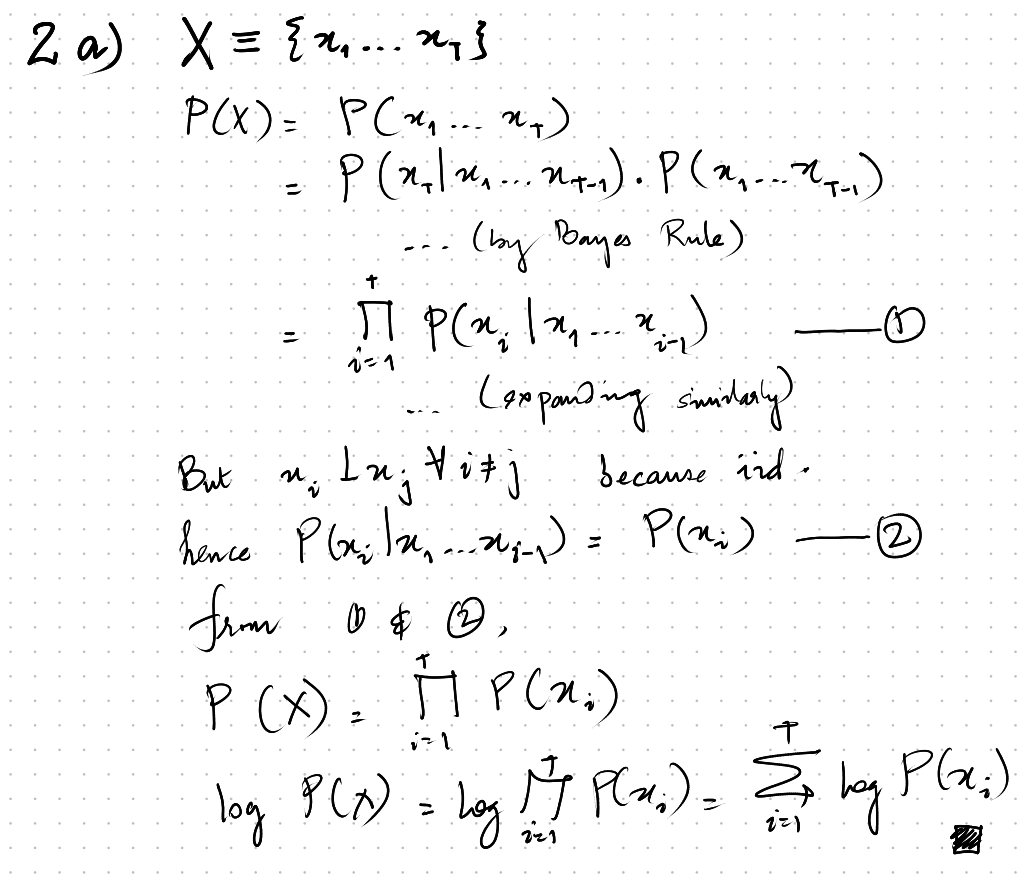
\includegraphics[width=.9\linewidth]{org-download-images/2024-11-12_10-15-18_screenshot.png}
\end{center}

\begin{center}
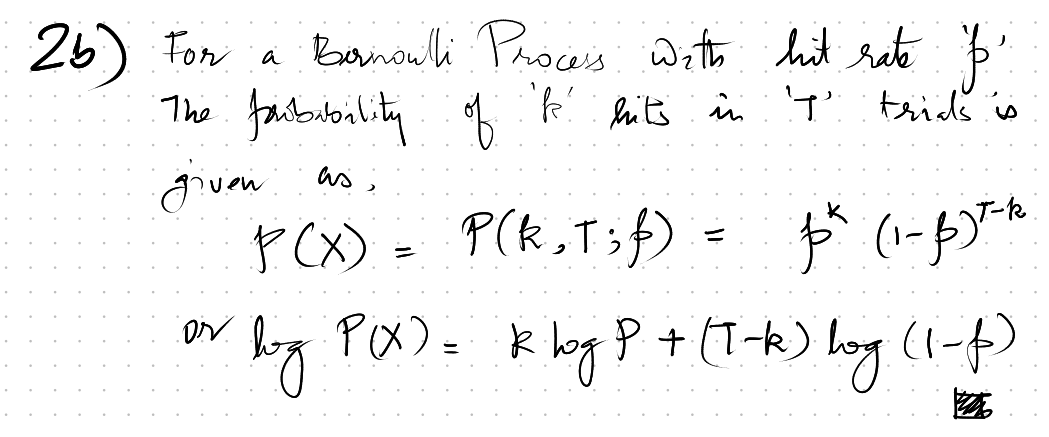
\includegraphics[width=.9\linewidth]{org-download-images/2024-11-12_10-18-39_screenshot.png}
\end{center}


\bvrskipline[0.25]
\begin{enumerate}[resume]
\item If \(X\equiv\{\mathbf{x}_1,\ldots,\mathbf{x}_T\}\) is
the temporal sequence of a Markov process, prove
that \(\log P(X) = \sum_{i=1}^T \log P(x_i\mid x_{i-1})\).
\end{enumerate}


\newpage
\bvrskipline[0.25]
{\huge

Speech sample \(X\) is a temporal sequence of intensities,

\begin{align*}
  X&\equiv\{x_1\ldots x_T\}
\end{align*}

Given speech samples \(\mathcal{D}\) as evidence,
estimate \(P_{\theta}\approx \mathcal{D}\) so that \(X\sim
P_\theta\) is a valid speech sample.

}

\newpage
\bvrhrule

{\huge

Let \(G_{\theta,\mathcal{N}} : \mathbb{X}^K \to
\mathbb{X}\) represent the model.

where,
\begin{itemize}
\item \(\mathbb{X}\) is the field of inputs.
\begin{itemize}
\item For a continuous model, \(\mathbb{X}\equiv
    \mathbb{R}\); whereas,
\item For categorical model,
\(\mathbb{X}\equiv\mathbb{R}_{[0,1]}^{256}\);
\item It may also be a hybrid model, \\[0pt]
\emph{e.g.} \(G_{\theta,\mathcal{N}} : \mathbb{R}^K \to
    \mathbb{R}_{[0,1]}^{256}\). \\[0pt]
Can you think how?
\end{itemize}
\end{itemize}

Let \(G_{\theta,\mathcal{N}} : \mathbb{X}^K \to
\mathbb{X}\) represent the model.

where,
\begin{itemize}
\item \(\mathcal{N}\) is a noise sampler,
\begin{itemize}
\item Generally, implemented as a normal distribution; or
\item Implemented implicitly as dropouts.
\end{itemize}
\end{itemize}

Let \(G_{\theta,\mathcal{N}} : \mathbb{X}^K \to
\mathbb{X}\) represent the model.

where,
\begin{itemize}
\item \(\theta\) are parameters of the model; and
\item \(\mathbf{x}_{t} = G_{\theta,\mathcal{N}}
  \left( \begin{bmatrix} \mathbf{x}_{t-K} & \ldots &
  \mathbf{x}_{t-1} \end{bmatrix} \right)\) models the
conditional distribution \(P(x_t \mid x_{t-K}\ldots
  x_{t-1})\)
\end{itemize}

\newpage

In case of Conditional Generation,

\(\mathbf{x}_{t} = G_{\theta,\mathcal{N}}
\left( \begin{bmatrix} \mathbf{x}_{t-K} & \ldots &
\mathbf{x}_{t-1} \end{bmatrix}, \mathbf{h} \right)\) \\[0pt]
models the conditional distribution \\[0pt]
\(P(x_t \mid x_{t-K}\ldots x_{t-1}, \mathbf{h})\)

\(\mathbf{h}\) represents the global conditions, \emph{e.g.}
\begin{itemize}
\item Text input;
\item Speaker;
\item Accent;
\item and so forth.
\end{itemize}

\newpage

Let \\[0pt]
\(X\equiv\begin{bmatrix} \mathbf{x}_1 & \ldots &
\mathbf{x}_T \end{bmatrix} \sim G_{\theta,\mathcal{N}}\)
be the output of the auto-regressive model, so that \\[0pt]
\(\mathbf{x}_{t} = G_{\theta,\mathcal{N}}
\left( \begin{bmatrix} \mathbf{x}_{t-K} & \ldots &
\mathbf{x}_{t-1} \end{bmatrix} \right)\)

\bvrskipline[0.25]

And, \\[0pt]
\(Y\equiv\begin{bmatrix} \mathbf{y}_1 & \ldots &
\mathbf{y}_T \end{bmatrix} \sim \mathcal{D}\) be a
speech sample from dataset.  Recall that for each time
step, the sound intensity is pre-processed so that the
values are remapped, quantised, and converted to
one-hot vectors, so that \(\mathbf{y}_t\in\{0,1\}^{256};
\|\mathbf{y}_t\|_{1}=1\) .

\bvrskipline[0.25]

The training objective is the cross entropy function,
given as,
\begin{align*}
  \underset{G}{\text{minimise}}\quad
  \underset{X\sim G, Y\sim\mathcal{D}}{\mathbb{E}}
  \left[ \sum_{i,t} y_{i,t}\log x_{i,t} \right]
\end{align*}


\newpage

\textbf{Tacotron}

\textbf{Artificial Neuron}

\begin{align*}
  \mathbf{y} &= \mathcal{N}(W\mathbf{x} + \mathbf{b})
\end{align*}

where,
\begin{itemize}
\item \(\mathbf{x},\mathbf{y}\in V\), for some vector space
\(V\);
\item \(W,\mathbf{b}\) are learnable weights; and
\item \(\mathcal{N}\) is a non-linearity applied
element-wise.
\end{itemize}

without loss of generality \\[0pt]
\textbf{ANN Layer}

\begin{align*}
  \mathbf{x}_{l+1} &= \mathcal{N}(W_l\mathbf{x}_l +
                     \mathbf{b}_l) 
\end{align*}

where,
\begin{itemize}
\item \(\mathbf{x}_{l}\in V \;\forall\, l\), for some vector space
\(V\);
\item \(W,\mathbf{b}\) are learnable weights; and
\item \(\mathcal{N}\) is a non-linearity applied
element-wise.
\end{itemize}

\textbf{Sequential Network} \\[0pt]
e.g. AlexNet, VGG Net etc.

\newpage

\begin{align*}
  \mathbf{y} &=\mathbf{g} \otimes \mathbf{x} \\
  \mathbf{g} &= \sigma(W\mathbf{x}+\mathbf{b})
\end{align*}
where,
\begin{itemize}
\item \(\otimes\) represents Hadamard product;
\item \(\sigma\) represents the logistic sigmoid function
that is applied element-wise; and
\item \(\mathbf{g}\in\mathbb{R}^n_{[0,1]}\) represents the
gate.
\end{itemize}


\textbf{Highway Gate}
\begin{align*}
  \mathbf{y} &= (\boldsymbol{1} - \mathbf{g}) \otimes
               \mathbf{x} + \mathbf{g} \otimes
               \mathbf{h} \\
  \mathbf{g} &= W_g\mathbf{x}+\mathbf{b}_g \\
  \mathbf{h} &= W_h\mathbf{x}+\mathbf{b}_h
\end{align*}


\textbf{Highway Gate}

In practice,
\begin{align*}
  \mathbf{y} &= (\boldsymbol{1} - \mathbf{g}) \otimes
               \mathbf{x} + \mathbf{g} \otimes
               \mathbf{h} \\
  (\mathbf{g},\mathbf{h})
             &= \left(\sigma
               (\widetilde{\mathbf{y}}_{:n}),
               \mathcal{N}
               (\widetilde{\mathbf{y}}_{n:}) \right) \\
  \widetilde{\mathbf{y}} &= W\mathbf{x}+\mathbf{b} 
\end{align*}

\newpage
\textbf{Constructing a highway network}

\(\forall\,l\in\{1,\ldots,L\}\)
\begin{align*}
  \mathbf{x}_{l} &= (\boldsymbol{1} - \mathbf{g}_l) \otimes
               \mathbf{x}_l + \mathbf{g}_l \otimes
               \mathbf{h}_l \\
  (\mathbf{g}_l,\mathbf{h}_l)
             &= \left(\sigma
               (\widetilde{\mathbf{x}}_{l,:n}),
               \mathcal{N}
               (\widetilde{\mathbf{x}}_{l,n:}) \right) \\
  \widetilde{\mathbf{x}}_l &= W_l\mathbf{x}_{l-1}+\mathbf{b}_l
\end{align*}

With \(L=50\) layer deep models, the very-deep network
building strategy shown here predates googlenet and
resnet.


\begin{align*}
P_\theta\left(Y|X\right)\quad\text{modelled as}\quad
  \mathbf{y} = G(\mathbf{x};\theta)
\end{align*}

as simple \\[0pt]
as possible

\begin{align*}
  P(\text{speech}\mid\text{text})
\end{align*}

\begin{align*}
  X\equiv\{\mathbf{x}_1\ldots\mathbf{x}_N\} \\
  Y\equiv\{\mathbf{y}_1\ldots\mathbf{y}_N\}
\end{align*}

\begin{align*}
P(x_i\mid x_1,…,x_{i-1},x_{i+1},...,x_T)
\end{align*}

}

\begin{center}
\begin{tabular}{|c|c|c|c|c|c|c|c|c|c|c|}
\hline
0.53 & 0.24 & 0.01 & 0.45 & 0.14 & 0.42 & 0.59 & 0.37 & 0.32 & 0.18 & 0.29\\[0pt]
\hline
0.56 & 0.16 & 0.32 & 0.44 & 0.32 & 0.63 & 0.52 & 0.85 & 0.75 & 0.75 & 0.33\\[0pt]
\hline
0.84 & 0.93 & 0.13 & 0.63 & 0.06 & 0.83 & 0.13 & 0.65 & 0.11 & 0.65 & 0.17\\[0pt]
\hline
0.92 & 0.62 & 0.08 & 0.13 & 0.18 & 0.72 & 0.83 & 0.54 & 0.83 & 0.29 & 0.45\\[0pt]
\hline
0.41 & 0.33 & 0.89 & 0.71 & 0.33 & 0.86 & 0.15 & 0.13 & 0.68 & 0.99 & 0.14\\[0pt]
\hline
0.26 & 0.17 & 0.03 & 0.48 & 0.29 & 0.40 & 0.60 & 0.27 & 0.85 & 0.66 & 0.11\\[0pt]
\hline
0.95 & 0.07 & 0.17 & 0.79 & 0.59 & 0.41 & 0.07 & 0.22 & 0.60 & 0.11 & 0.11\\[0pt]
\hline
0.27 & 0.72 & 0.02 & 0.97 & 0.62 & 0.53 & 0.49 & 0.81 & 0.00 & 0.29 & 0.52\\[0pt]
\hline
0.88 & 0.17 & 0.24 & 0.77 & 0.59 & 0.40 & 0.71 & 0.88 & 0.07 & 0.21 & 0.17\\[0pt]
\hline
0.23 & 0.06 & 0.48 & 0.97 & 0.18 & 0.85 & 0.62 & 0.82 & 0.73 & 0.66 & 0.70\\[0pt]
\hline
0.67 & 0.66 & 0.24 & 0.46 & 0.19 & 0.87 & 0.83 & 0.19 & 0.15 & 0.21 & 0.70\\[0pt]
\hline
0.28 & 0.72 & 0.32 & 0.04 & 0.48 & 0.16 & 0.47 & 0.34 & 0.52 & 0.14 & 0.75\\[0pt]
\hline
0.94 & 0.73 & 0.20 & 0.57 & 0.68 & 0.47 & 0.90 & 0.54 & 0.67 & 0.18 & 0.84\\[0pt]
\hline
\end{tabular}
\end{center}

\vfill
\bvrhrule
\bvrskipline[-0.85]
\bvrhrule
\end{document}
